\documentclass{bredelebeamer}

\usepackage{minted}
\usepackage{listings}
\usepackage{svg}
\usepackage{environ}

\title[Train planning in OSRD]{Automated short-term train planning in OSRD: from POC to production}
\subtitle{}
\author{Eloi Charpentier - SNCF Réseau}
\date{}

\subject{Train planning in OSRD}

\begin{document}

\begin{frame}
  \titlepage
\end{frame}


\begin{frame}{OSRD (Open-Source Railway Designer)}
	\begin{itemize}
		\item OSRD is an open-source project that can be used to \textbf{edit railway infrastructures} and \textbf{run simulations}.
		\item We'll talk about one of its many features:\\ \textbf{train planning}.
	\end{itemize}
	\begin{center}
		\includesvg[height=30px]{img/svg/logos/osrd_small}
		\includesvg[height=40px]{img/svg/logos/sncf-reseau}
		\vspace{0.5cm}\\
		\includesvg[height=30px]{img/svg/logos/rust}
		\includesvg[height=30px]{img/svg/logos/kotlin}
		\includesvg[height=30px]{img/svg/logos/typescript}
	\end{center}
\end{frame}

\section{Problem presentation}
	\begin{frame}{Problem presentation}
		\begin{block}{}
			A train wants to go from Station A to Station B, leaving tomorrow.
			We're the railway infrastructure manager and need to find a way.
		\end{block}
		\vspace{1cm}
		\includesvg[width=\textwidth]{img/svg/examples/1}
	\end{frame}
	
	\begin{frame}{Problem presentation}
		\begin{block}{}
			But many trains have already been scheduled!\\
			(10k to 15k per day)
		\end{block}
		\vspace{1cm}
		\includesvg[width=\textwidth]{img/svg/examples/2}
	\end{frame}
	
	\begin{frame}{The rules}
		We cannot:
		\begin{itemize}
			\item Delay scheduled trains
			\item Provide an unrealistic path
		\end{itemize}
		We can:
		\begin{itemize}
			\item Add \textbf{detours}
			\item Slow down the new train
			\item Change the departure time
			\item Add or lengthen stops
		\end{itemize}
	\end{frame}
	
	\begin{frame}{Search space}
		\begin{block}{}
			We now have a complex search problem in space and time. On one given path:
		\end{block}
		
		\includegraphics[scale=0.25]{img/png/space-time-chart.png}
	\end{frame}
	

\section{The original POC}

	\begin{frame}{Our solution: general principles}
		
		\begin{block}{}
			We evaluate one big \textbf{decision tree}:\\
			we enumerate all possible solutions and run a pathfinding algorithm on that tree (A*).\\
			First on space:
		\end{block}
		
		\includesvg[width=180px]{img/svg/examples/infra-decision-tree}
	\end{frame}
	
	\begin{frame}{Our solution: general principles}
		
		\begin{block}{}
			Then on top of each path, we evaluate another decision tree along the time axis:
		\end{block}
		
		\includesvg[width=250px]{img/svg/examples/space-time-chart-decision-tree}
	\end{frame}


\section{Short demo}
	\begin{frame}{Short demo}
		\begin{block}{}
			(recorded demo here: it shows the paths being explored on the map, and a resulting space time chart)\\
			
			link to mkv file: \url{https://github.com/eckter/fosdem\_2026/blob/master/short\_demo.mkv}\\
			
			TODO: remove this text
		\end{block}

	\end{frame}


\section{Deployment and new challenges}

	\begin{frame}{How the new tool fits in the existing processes}
		\begin{block}{}
				People are in charge of answering such requests: timetable planners
		\end{block}
		
		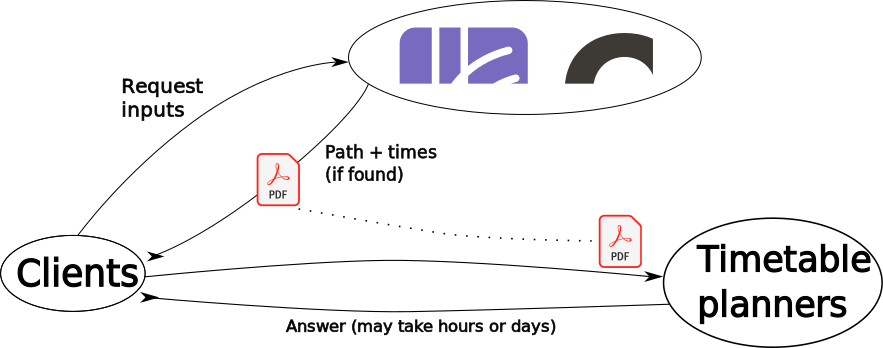
\includegraphics[scale=0.40]{img/png/interactions.png}
	\end{frame}
	
	\begin{frame}{Early 2025 : real data and first users}
		\begin{itemize}
			\item First requirement: data
			\item We first focused on a specific axis
			
			
			\includesvg[height=150px]{img/svg/examples/perimeter}
		\end{itemize}
	\end{frame}
	
	\begin{frame}{Early 2025 : first users and feedback}
		\begin{itemize}
			\item First feedback from the new users!
			\item They want to use it as an optimistic \textbf{pre-filtering} check: "is there a chance my request could be accepted?"
			\item ...But we were on the pessimistic side.
			\item We then rushed some new features to fix that (e.g. adding extra stops).
		\end{itemize}
	\end{frame}
	
	
	\begin{frame}{2025 : feedback from timetable planners}
		\begin{itemize}
			\item They had data issue with \textit{specific} examples.
			\item We had to work on our logging and context saving.
			\item They don't focus on the same kind of data!
			\item Sometimes explaining \textbf{why} our solution was wrong could be difficult.
		\end{itemize}
	\end{frame}
	
		
	\begin{frame}{Some numbers}
		\begin{itemize}
			\item We receive 10 to 20 requests per day
			\item Only a few are actually forwarded to timetable planners with the PDF file (1-2 per week)
			\item Out of those:
			\begin{itemize}
				\item \textbf{13\%} false positives
				\item \textbf{6\%} false negatives
				\item All of the identified errors come from data issues
			\end{itemize}
			\item Computation time per request: from 200ms to 3 minutes, 16s average
		\end{itemize}
	\end{frame}




\section{Conclusion}
	\begin{frame}{What we've learned}
		\begin{itemize}
			\item The technical approach is sound
			\item The hard part is the data quality, not just the algorithm
			\item There's a lot of people we need to convince
		\end{itemize}
		\begin{block}{}
			It can work on any infrastructure as long as there's data.\\
			We're always looking for collaborators, feedback, or other infrastructure managers interested in trying this
		\end{block}
	\end{frame}
	\begin{frame}{Questions}
		\Large Any question?
		\normalsize

		\vspace{2cm}

		For more information: \url{https://osrd.fr}\\
		Github: \url{https://github.com/OpenRailAssociation/osrd}\\
		Chat with us: \url{https://matrix.osrd.fr}\\
		Email: \url{contact@osrd.fr}
	\end{frame}

\end{document}
